% Part: sets-functions-relations
% Chapter: arithmetization
% Section:reals

\documentclass[../../../include/open-logic-section]{subfiles}

\begin{document}

\olfileid{sfr}{arith}{real}
\olsection{বাস্তব সংখ্যারেখা}

পরের ধাপে মূলদ সংখ্যা থেকে বাস্তব সংখ্যা কীভাবে নির্মাণ করা যায় তা দেখাতে হবে। তার আগে বাস্তব সংখ্যার \emph{বিশিষ্ট} বৈশিষ্ট্যটি বুঝতে হবে।

বাস্তব সংখ্যার আচরণ মূলদ সংখ্যার খুবই অনুরূপ। (কারিগরি ভাষায়, উভয়েই \emph{ক্রমিত ক্ষেত্র}-এর উদাহরণ; এর সংজ্ঞার জন্য \olref[check]{orderedfield} দেখো।) এখন, তুমি যদি \olref[sfr][siz][]{chap}-এর অনুশীলনগুলি করে থাকো, তবে জানবে যে মূলদ সংখ্যার চেয়ে বাস্তব সংখ্যা প্রকৃতই বেশি, অর্থাৎ $\cardless{\Rat}{\Real}$। কান্টর প্রথম এটি প্রমাণ করেছিলেন। কিন্তু প্রায় আড়াই সহস্রাব্দ ধরে জানা আছে যে অমূলদ সংখ্যা আছে, অর্থাৎ এমন বাস্তব সংখ্যা যা মূলদ নয়। বস্তুত:
%\footnote{এখন: ``$\sqrt{2}$'' একইভাবে ধনাত্মক ও ঋণাত্মক মূল উভয়কেই বোঝায়; কিন্তু পরের কয়েকটি পৃষ্ঠায় আমি এ কথা ভুলে গিয়ে শুধু ধনাত্মক মূলটি বিবেচনা করব।}
\begin{thm}\ollabel{root2irrational}
$\sqrt{2}$ মূলদ নয়, অর্থাৎ $\sqrt{2} \notin \Rat$
\end{thm}

\begin{proof}
স্ববিরোধে উপনীত হওয়ার জন্য ধরি, $\sqrt{2}$ মূলদ। তাহলে কোনো স্বাভাবিক সংখ্যা $m$ ও $n$-এর জন্য $\sqrt{2} =
\nicefrac{m}{n}$। বস্তুত, আমরা $m$ ও $n$-কে একই সঙ্গে যত ছোট সম্ভব বেছে নিতে পারি, ফলে ভগ্নাংশটিকে আর লঘিষ্ঠ করা যায় না। % BN-SRC-008 TARGET-CORRECTION-BEGIN
\par\smallskip\noindent\textnormal{\small\textbf{উৎস-ব্যাখ্যা (BN-SRC-008):} হিমায়িত ইংরেজি উৎস প্রথমে শুধু ভগ্নাংশটি আর লঘিষ্ঠ করা যায় না বলে, কিন্তু জ্যামিতিক যুক্তির শেষে $m$ ও $n$-কে ``যত ছোট সম্ভব'' ধরে বিরোধ আনে। বৈধ অসীম-অবতরণ যুক্তিতে শুরুতেই একটি সর্বনিম্ন প্রতিনিধিত্ব বেছে নেওয়া যায়; বাংলা পাঠে সেই প্রয়োজনীয় নির্বাচনটি স্পষ্ট করা হয়েছে।} % BN-SRC-008 TARGET-CORRECTION-END
পুনর্বিন্যাস করলে $m^{2} = 2n^{2}$। এখান থেকে আমরা দুইভাবে প্রমাণটি সম্পূর্ণ করতে পারি:

\emph{প্রথমত, জ্যামিতিকভাবে} (টেনেনবাউমকে অনুসরণ করে)।\footnote{এই প্রমাণটি \cite{Conway2006}-এ উল্লেখ করা হয়েছে।} নিচের বর্গগুলি বিবেচনা করো:
\begin{center}
	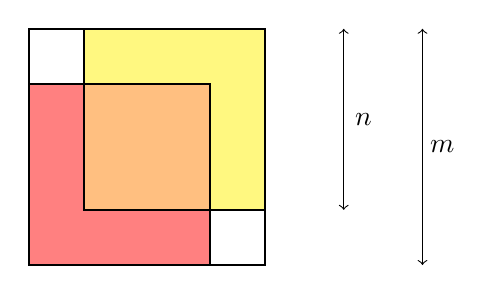
\begin{tikzpicture}
		\draw[thick] (0,0) rectangle (3,3);
		\draw[thick, fill=red!50] (0,0) rectangle (2.3,2.3);
		\draw[thick, fill=yellow!50] (0.7,0.7) rectangle (3, 3);
		\draw[thick, fill=orange!50] (0.7,0.7) rectangle (2.3, 2.3);
		\draw[<->] (4, 0.7)--(4, 3);
		\node at (4.25, 1.85) (n) {$n$};
		\draw[<->] (5, 0)--(5, 3);
		\node at (5.25, 1.5) (m) {$m$};
	\end{tikzpicture}
\end{center}
$m^2 = 2n^2$ বলে $n$ বাহুবিশিষ্ট বর্গদুটির অধিক্রমণ অঞ্চলটির ক্ষেত্রফল, বর্গদুটি যে অঞ্চল ঢাকে না তার ক্ষেত্রফলের সমান; অর্থাৎ কমলা বর্গটির ক্ষেত্রফল ছায়াহীন বর্গদুটির ক্ষেত্রফলের যোগফলের সমান। তাই কমলা বর্গের বাহু $p$ এবং প্রতিটি ছায়াহীন বর্গের বাহু $q$ হলে, $p^2 = 2q^2$। কিন্তু তখন $\sqrt{2} = \nicefrac{p}{q}$, যেখানে $p < m$, $q < n$ এবং $p, q \in
\Nat$। এটি $m$ ও $n$-কে যত ছোট সম্ভব বেছে নেওয়ার বিরোধী।

\emph{দ্বিতীয়ত, আনুষ্ঠানিকভাবে।} $m^{2} = 2n^{2}$ বলে $m$ জোড়। ($x$ বিজোড় হলে $x^2$-ও বিজোড়—এটি সহজেই দেখানো যায়।) তাই কোনো $r \in \Nat$-এর জন্য $m = 2r$। পুনর্বিন্যাস করলে $2r^2 = n^2$,
		%			\begin{align*}
		%				(2q)^{2} &= 2n^{2}\\
		%				4q^{2} &= 2n^{2}\\
		%				2q^{2} &= n^{2}
		%			\end{align*}
তাই $n$-ও জোড়। অতএব $m$ ও $n$ উভয়েই জোড়, আর সেই কারণে ভগ্নাংশ $\nicefrac{m}{n}$-কে আরও লঘিষ্ঠ \emph{করা যায়}। স্ববিরোধ!
\end{proof}

প্রসঙ্গত, এই চিত্রভিত্তিক প্রমাণটি আমাদের \olref[his][set][mythology]{sec}-এর আলোচনায় ফিরে যাওয়ার সুযোগ দেয়। টেনেনবাউম (1927--2006) পুরোপুরি আধুনিক গণিতবিদ ছিলেন; তবু প্রমাণটি নিঃসন্দেহে সুন্দর, সম্পূর্ণ নিখুঁত এবং জ্যামিতিক স্বজ্ঞাকে কাজে লাগায়!

যাই হোক, বাস্তব সংখ্যাগুলি মূলদ সংখ্যার তুলনায় ``আরও বিস্তৃত''। এক অর্থে মূলদ সংখ্যার মধ্যে ``ফাঁক'' আছে, এবং বাস্তব সংখ্যা সেই ফাঁকগুলি পূরণ করে। ভাইয়ারস্ট্রাস উপলব্ধি করেছিলেন যে এটি বাস্তব সংখ্যার এমন একটি একক বৈশিষ্ট্য বর্ণনা করে, যা তাদের মূলদ সংখ্যা থেকে পৃথক করে; বৈশিষ্ট্যটি হলো পূর্ণতা ধর্ম: \emph{বাস্তব সংখ্যার প্রত্যেক অশূন্য সেটের একটি ঊর্ধ্বসীমা থাকলে তার একটি লঘিষ্ঠ ঊর্ধ্বসীমা আছে।}

মূলদ সংখ্যার যে পূর্ণতা ধর্ম নেই, তা সহজেই দেখা যায়। যেমন, $\sqrt{2}$-এর চেয়ে ছোট মূলদ সংখ্যাগুলির সেটটি বিবেচনা করো, অর্থাৎ:
\[
	\Setabs{p \in \Rat}{p^2 < 2 \text{ অথবা }p < 0}
\]
মূলদ সংখ্যার মধ্যে এই সেটটির একটি ঊর্ধ্বসীমা আছে; যেমন, এর !!{element}s সকলেই $3$-এর চেয়ে ছোট। % BN-SRC-007 TARGET-CORRECTION-BEGIN
\par\smallskip\noindent\textnormal{\small\textbf{উৎস-সংশোধন (BN-SRC-007):} হিমায়িত ইংরেজি উৎসে টোকেনটির ঠিক পরে একটি অর্থহীন অতিরিক্ত ``<'' অক্ষর আছে। বাংলা পাঠে সেটি বাদ দেওয়া হয়েছে; কোনো সূত্র বা অসমতা পরিবর্তিত হয়নি।} % BN-SRC-007 TARGET-CORRECTION-END
কিন্তু এর লঘিষ্ঠ ঊর্ধ্বসীমা কী? আমরা বলতে চাই `$\sqrt{2}$'; কিন্তু এইমাত্র দেখেছি যে $\sqrt{2}$ মূলদ \emph{নয়}। আবার $\sqrt{2}$-এর চেয়ে বড় কোনো \emph{লঘিষ্ঠ} মূলদ সংখ্যাও নেই। তাই সেটটির একটি ঊর্ধ্বসীমা আছে, কিন্তু কোনো লঘিষ্ঠ ঊর্ধ্বসীমা নেই। সুতরাং মূলদ সংখ্যার পূর্ণতা ধর্ম নেই।

অন্যদিকে, সতত সমষ্টির পূর্ণতা ধর্ম থাকা ``নৈতিকভাবে উচিত''। আমরা শুধু $\sqrt{2}$-কে বাস্তব সংখ্যা হিসেবে পেতে চাই না; মূলদ সংখ্যারেখার সব ``ফাঁক'' পূরণ করতে চাই। বস্তুত, সতত সমষ্টির নিজের মধ্যেই কোনো ``ফাঁক'' চাই না। পূর্ণতার সাহায্যে আমরা ঠিক এটিই পাব।

\end{document}
